\documentclass[uplatex]{jsreport}
\usepackage{docmute}
\usepackage{myStyle}
\label{chapterXX}

\begin{document}

\chapter{帰無仮説検定の実際}
前回は，帰無仮説と対立仮説という二つのモデルを戦わせる意思決定法，帰無仮説検定のやり方について導入的なお話をしました。今回は，これをいくつかの具体例に当てはめて考えていくことにしましょう。具体的な計算式や確率的な数字は，統計パッケージで児童的に計算されます。その利便性のおかげで，帰無仮説検定がさまざまな学問領域に広く行き渡ったことは既に指摘した通りですが，同時に「手続きが簡単だから，内容も簡単」だと思っていると，誤用・開くようになりますので，よく注意してください。例えるなら，車の運転がマニュアルトランスミッションからオートマチックになったことで，比較的簡単に運転できるようになりましたが，それで交通量が増えて事故が多発するようでは，かえって社会的には良くないことかもしれない，ということです\footnote{電子レンジの普及のように，簡単になって利便性が増し，危険性もそうない技術的なものもあります。車の例えも，危険性と利便性のバランスでいくと，十分許容範囲なのかもしれませんが，帰無仮説検定は利便性も危険性もどちらも大きい，ハイリスク・ハイリターンな技術なのです。}
\section{一つの平均値の検定}
\subsection{母SDがわかっている場合}
ではまず，一つの平均値の推定を使って，検定をしてみましょう。「推定を使って検定」というのは変な表現に聞こえるかもしれませんが，推定は「母数はこれぐらいではないか」という予測の話であり，検定は「母数がそのようであれば，このように結論づける」という意思決定の話なのです\footnote{意思決定なんかしなくていいじゃない，と思うかもしれません。確かに科学的探究であれば，母数がどの程度であるかというのを知ることで十分なのです。しかし，帰無仮説検定は農学で生まれ，医学領域にも広まっている技術です。これ以上実験を続けて良いかどうか，この治療薬を投与し続けて良いかどうか，といった実際的な問題がそこにはあり，効果があるとしたらこれぐらい，ない可能性もなくはない...という態度を続けていると前に進まないので，何らかの基準が必要だという事情もあります。心理学においても，より実際的な場面では意思決定が必要になることもありましょう。}。

され話を進めるために，具体的な例をあげてみましょう。ある学校で，学力テストしたとします。その学校で無作為に49人分の記録を取り出したところ，平均が52点でした。このテスト，全国平均は50点で，SDが9の正規分布であることがわかっていたとします。これとそのまま比べると，その学校の成績が良い，ということになりますが，たった2点差でそのように結論づけて良いかどうか，というのがここでの仮定です。

帰無仮説検定のステップを思い出しましょう。まずは仮説を設定します。帰無仮説は，「その学校の成績が特段良いわけではない」であり，対立仮説は「この学校は特別で，成績が良い」になります\footnote{これらの仮説は，母平均についてのものです。その学校には他にもたくさんの生徒がおり，全員分のテストを取り出したわけではない，という設定です。つまり，母集団はその学校全体の平均値であり，母集団も正規分布していて，母平均$\mu$と母分散$\sigma^2$で特徴づけられる世界です。これが理論的な正規分布と合うかどうか，という話をしています。}。

次に検定統計量ですが，平均値の推定，しかも理論的に平均50，SD9の正規分布との照合ですから，推定したい対象の特徴がもうわかっている特殊なケースです。これは変換すれば標準正規分布に従うのですから($\to$\ref{chapter16})，標準化されたZ得点が検定統計量になります。

第3のステップは基準になる確率を設定する，でした。勝敗を決めるルールの決定ですね。これは特に意味もなく，慣例に従って0.05(5\%)としておきましょう。

これで準備が終わりました。実際の検定統計量の計算です。平均$\mu$，分散$\sigma^2$の正規分布する母集団からの標本の場合，標本平均の標本分布も正規分布に従い，
$$ \bar{X} \sim N(\mu,\frac{\sigma}{\sqrt{n}}) $$
になります。今回の場合は，
$$ 52 \sim N(50,9/\sqrt{49}) $$
だと考えられます。標準化することで標準正規分布を使うことができますから，
$$ (52-50)/(9/7) \sim N(0,1) $$
として，$ (52-50)/(9/7) =2/1.285714=1.555... $を得ます。この1.556(下三桁までで四捨五入しました)という数字はどのあたりに位置するのでしょう？

そこで確率の計算をしてみましょう。これが次のステップの，実際のデータから検定統計量の実現値を計算する，というやつです。標準正規分布において，1.556より大きな数字が得られる確率は\footnote{これまた確率の，特に連続変数のややこしいところで，1.556という数字が出てくる確率はゼロです。ユークリッド幾何学でいうところの，点は位置があって大きさがないというのと同じで，点の確率は大きさがないのです。確率は面積ですから，1.556\underline{より大きな数字}が得られる確率，という表現にしなければなりません。}，$p=0.05985405$でした\footnote{これはRで次のように計算しています：\texttt{1-pnorm(1.556,mean=0,sd=1)}}。5.9\%なのですね。

最後に判定です。5\%が判定ラインだったわけですが，今回得られた「確率変数の実現値」は5\%より大きな確率です。つまり大きい＝出現する可能性が大きい，よくある話だったわけです。そんなにレアな数字じゃない。つまり，たまたま今回の標本が，平均から2点大きくなるようなことは十分あり得る話だということです。この学校の生徒は優秀だー！と言いたいところなんですが，偶然それぐらいの差がでることがあるのであれば，そこまで胸を張っていうことができません。ということで，軍配としては帰無仮説の勝ち，つまり，「その学校の成績が特段良いわけではない」「統計的には差がない」ということになります。

\subsection{母SDがわかっていない場合}
先ほどの例は，母SDがわかっているという話でした。第\ref{chapter17}講でも同じことを言いましたが，まあ母数がわかっていれば苦労はないわけで，それが分からないから推測するのですよね。

ということで，母SDの代わりに標本SD(不偏分散の正の平方根)を使って推定することとします。そのさいは(標準)正規分布が使えないので，サンプルサイズに応じた$t$分布を使うのでした。同じデータ例でやってみましょう。今度は標本標準偏差が必要ですので，これが$\hat{\sigma}=10$だったとします。

帰無仮説・対立仮説は同じです。検定統計量が$t$になるわけです。
判断基準も同じく慣例にならって，なんとなく5\%にしておきましょう。
検定統計量$t$は$t = \frac{\bar{X}-\mu}{\hat{\sigma}/\sqrt{n}}$で求めることができますから，
$$ t = (52-50)/(10/7) = 1.4 $$
となります。これが自由度$n-1=48$の$t$分布に従うので，自由度48の$t$分布において1.4以上の数字が出る確率を求めますと，$p=0.08397194$となりました\footnote{これはRで次のように計算しています：\texttt{1-pt(1.4,df=48)}}。8.3\%なのですね。

これで判定です。5\%の判定ラインより大きな確率が出ましたので，これは滅多にないことではない。なくはないのだから，よくある話。珍しいことじゃない。つまり，母平均から外れて大きい数字，とまでは言えないねということになります。

いかがでしたでしょうか。今回のデータでは(母SDがわかっていても，わかっていなくても)帰無仮説を棄却することはできませんでした。何だか持って回った言い方をしているように感じられるかもしれませんし，いまいちイメージが掴みにくいかもしれません。そこで，今度はまた別のケース，相関係数の例で考えてみたいと思います。徐々に手続きと結論の出し方に慣れていくと思います。

\section{相関係数の検定}
今度は相関係数の検定の話をしましょう。
心理学では，平均値を推測するだけでなく，相関係数をテーマに研究することも少なくありません。実験など，介入の前後や群間の比較であれば平均値の話になりますが，こうした因果関係が明確でなく，何らかの関係があるかもしれない，という見込みで探索的に現象を解明していくこともよくあります。例えばうつ病と起床時間に関係があるのかもしれない。自尊心の高さは学業成績と関係があるのかもしれない。恋愛に対する態度には性格が関係しているのかもしれないetc...。何だか心理学っぽい話になってきましたね！

さて最後の例，恋愛に対する態度と性格の関係，を研究したいとしましょう。先行研究から，「恋愛についての積極性」を測定する尺度と，外交的な性格かどうかを測定する尺度があったとします\footnote{ここでは軽〜く書いていますが，心理的な状態を測定する物差しのことを\keyterm{尺度}scaleといい，この尺度を作る・使い方を考えるのも心理学の重要な研究領域なのです。この領域を特に「心理測定」といいますが，テスト理論の発展系である因子分析モデルや構造方程式モデリングによって，調査項目に対する反応を細やかに検証する世界があります。それでなくても目に見えないものを測定するのですから，きちんと測定できているかどうか--信頼性と妥当性($\to$第\ref{chapter05}講)は大問題です。また世の中には論文化され，公開されている心理尺度はたくさんありますが，自分の研究に借用するときは「本当に自分が測りたいものと，この尺度が測ろうとするものが同じなのか」「今の，私の研究対象に同じ測定方法で測って同じ結果が得られるのか」，など常に批判的な態度を持っておく必要があります。}。この尺度を使って，協力者を20人募って回答を求め，標本相関係数を算出したところ，$r=0.5$という数字が得られたとします(相関係数の算出については$\to$第\ref{chapter03}講)。

さて，標本相関係数は$r=0.5$ですが，母相関係数はどうでしょうか。母集団でもこの2変数は関係がある，と言って良いでしょうか。標本の話を母集団に広めるには推定，そして結論づけるには検定をするのでした。検定のステップを踏んで話を進めましょう。

\paragraph{仮説の設定：相関係数の場合}
まずは仮説の設定です。帰無仮説と対立仮説が必要なのでした。帰無仮説はNullな仮説ですから，今回は「相関関係がない」というのがそれになります。
母相関はギリシア文字$\rho$(ローとよむ)で表されますから，数学的な表現をすると帰無仮説は$H_0: \rho =0$です。母相関が$0.0$と一致する，という強い主張ですね。
これに対する対立仮説は，これの否定ですから$H_1:\rho \neq 0$です。既にこの2つのモデル対決，帰無仮説はピンポイント予測ですから，かなり狭い可能性のような気もしますが，帰無仮説検定の話の上ではこうならざるを得ないのです。

というのも，帰無仮説検定は背理法のロジックを使う，というところにその話の味噌があります。まずは極端かもしれませんが，帰無仮説の世界を想定しておき，それに従っていくとおかしなことが起こるなら，帰無仮説を棄却する，という話の進め方です。母相関が0な世界を想定してみましょう--幸い，最近はコンピュータを使って簡単にシミュレーションをすることができます。相関係数が0の世界があり，そこから20人のサンプルをとっていくとしましょう。

\begin{figure}[ht]
    \centering
    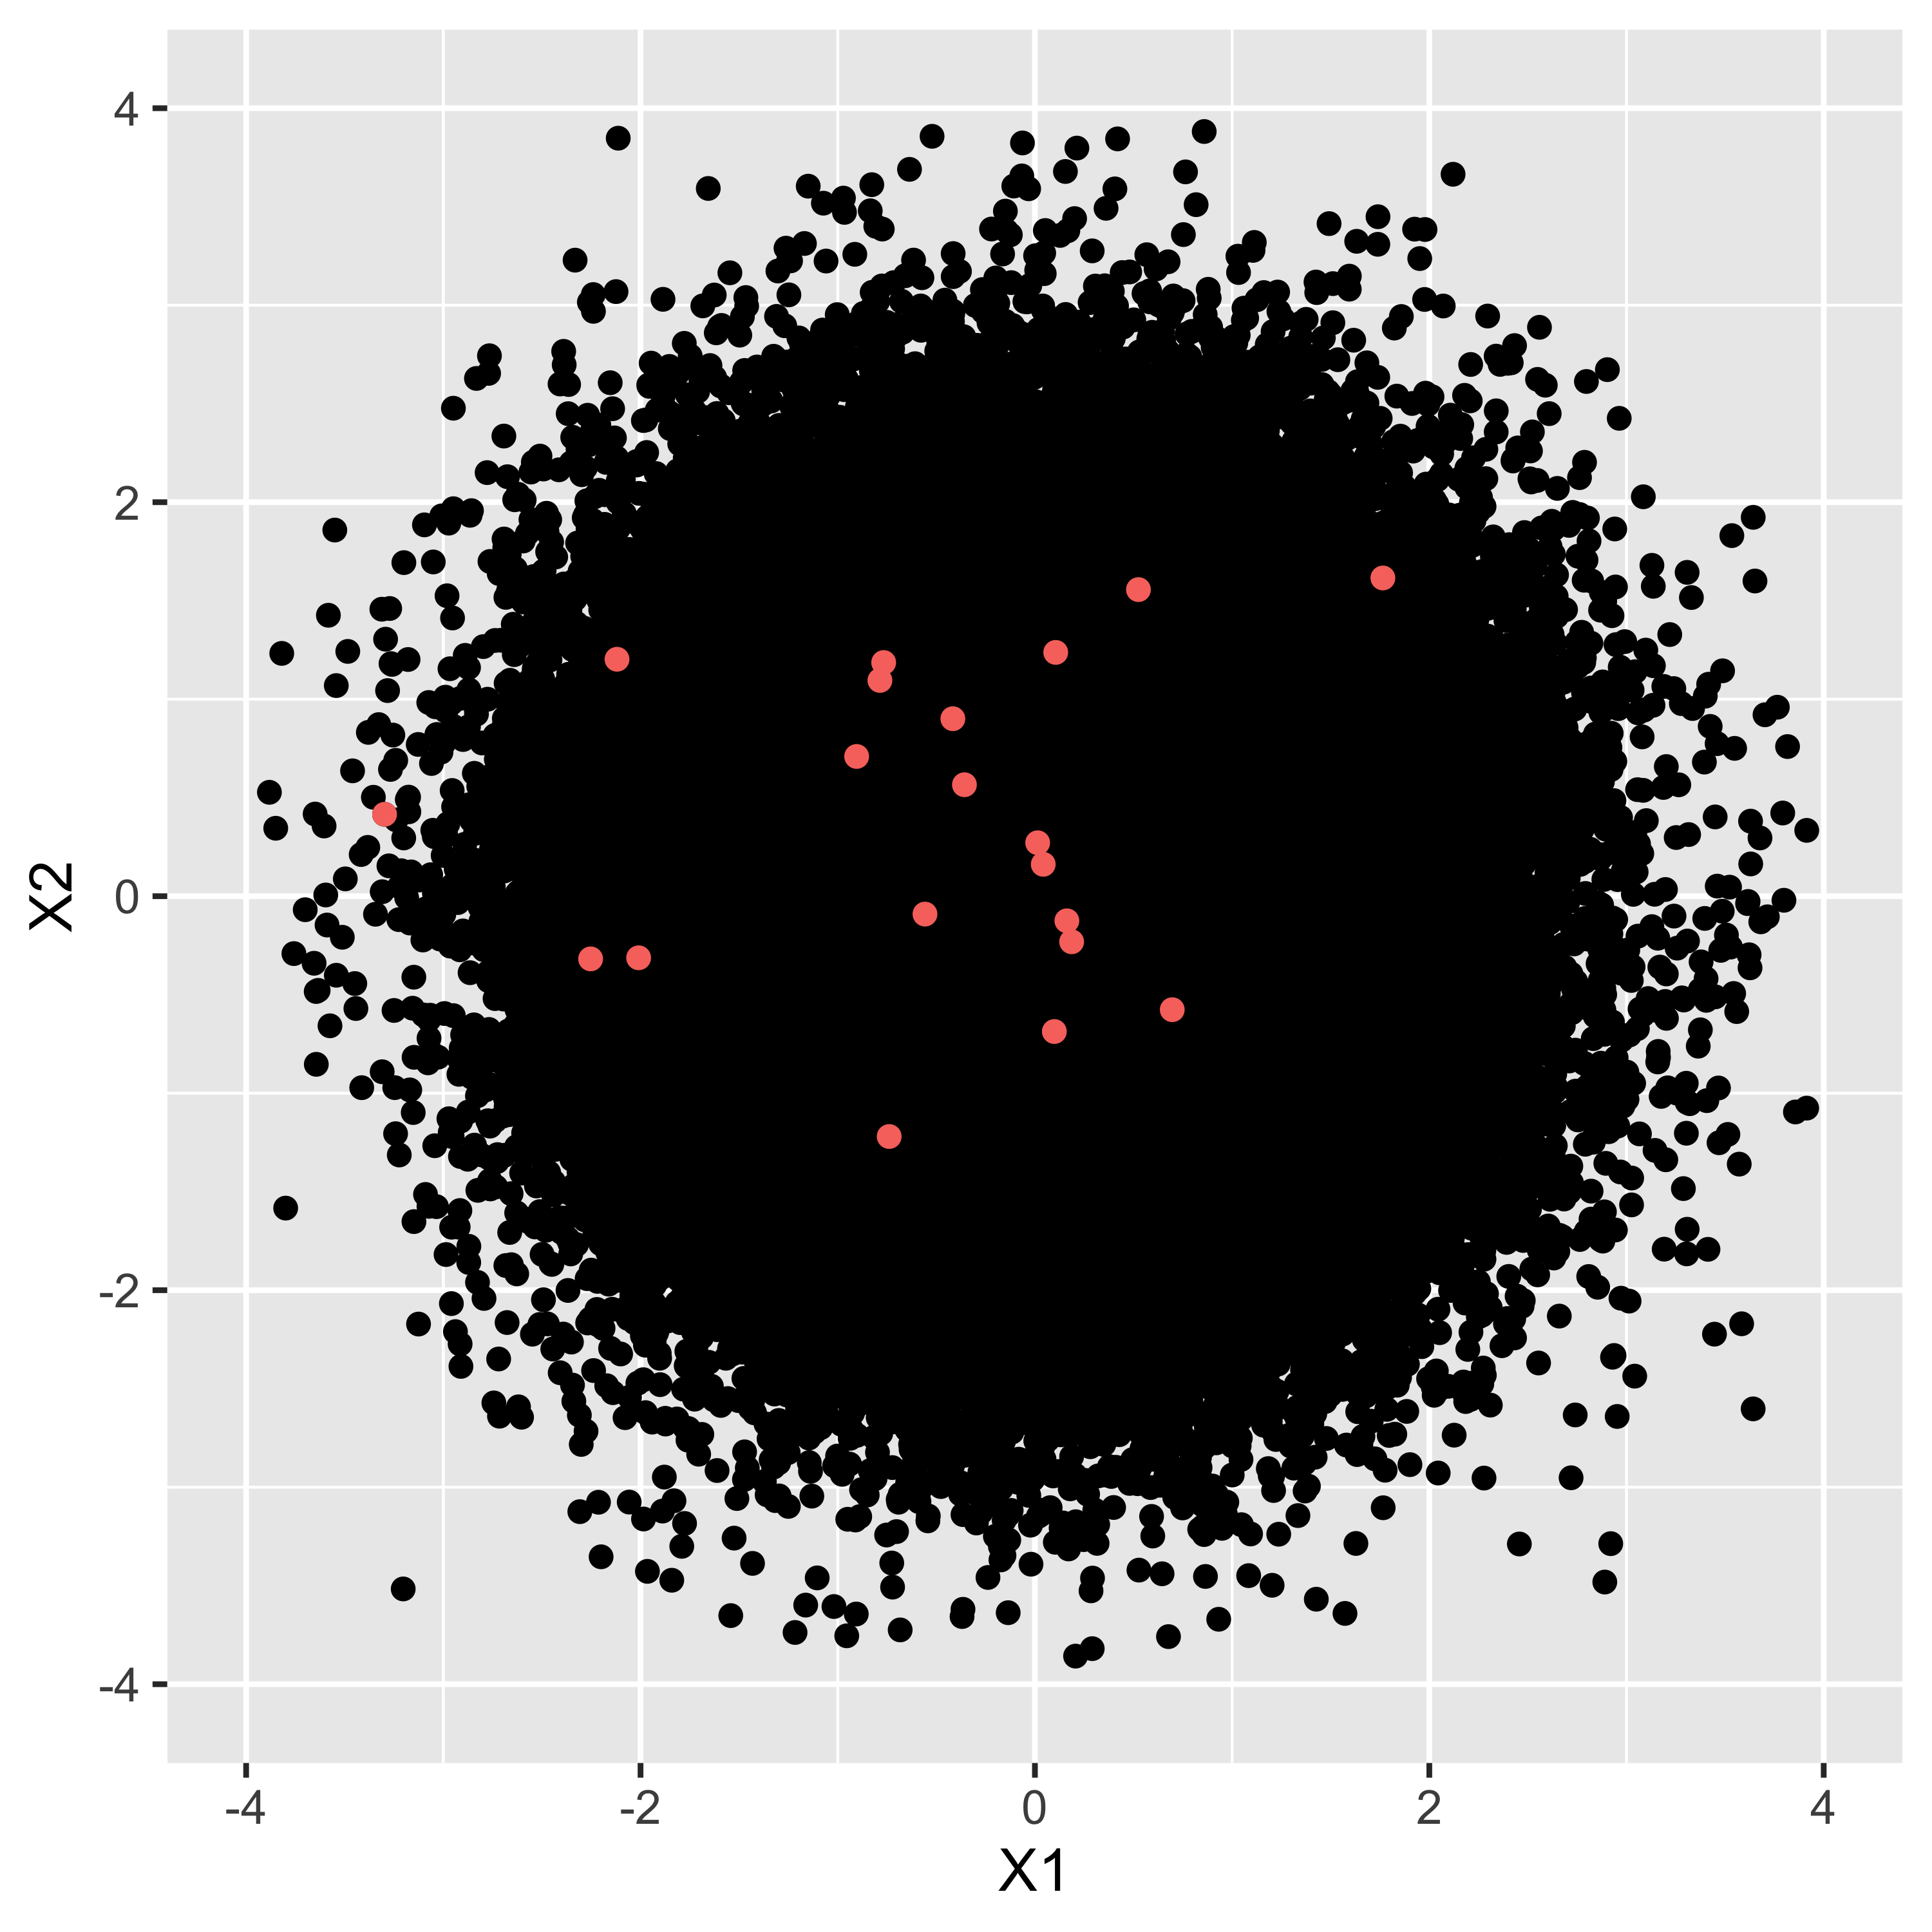
\includegraphics[keepaspectratio,width=12cm]{images/text18/Rplot18_01.png}
    \caption{母相関$\rho=0$の世界とそこから$n=20$のサンプルを取った例}
    \label{fig::18_01}
\end{figure}

図\ref{fig::18_01}に示したのは，母相関$\rho=0$の世界から乱数を10万点発生させ，そこからランダムに20個の点を取り出した例です。黒い点の塊はほぼ円で，二変数に相関がないというデータを具現化したものが示されています。小さな赤い点がそこから20個取り出した場合で，今回この20個の点による標本相関係数は$r=0.143$でした。理論的には$\rho=0$の世界からのサンプルなのですから，$r$も0であって欲しいかもしれませんが，一部の標本だけ取り出すとぴったり0になることはありません。同様のサンプルを何度も繰り返すと，標本相関係数は$r_2=0.32, r_3=-0.46,r_4=-0.26....$といろいろな数字を取ります。この分布が標本分布になるのです。

このように，一旦「母相関は$\rho=0$」，としてから標本を取り出したとして，その標本分布がどうなるかを考え，たまたま今回得られた標本相関係数(今回の例では0.5でしたが)が出てくる確率はどれぐらいか，を考えます。その確率が非常に小さければ，滅多にないことが目の前のデータで生じたわけですから，これは前提である「母相関は$\rho=0$」という仮定の方がおかしい，ということで帰無仮説を捨てるわけです。ここが背理法になっているわけですね。また，帰無仮説として「母相関はありまぁす！」という仮定を置くのも難しいところなのがわかっていただけるかと思います。相関が「ある」といって，どの程度あるのかは無数に考えられるのに対し，相関が「ない」の場合は一位に定まるからです。

\paragraph{検定統計量を定める}

ここで，標本相関係数の標本分布は，自由度$n-2$の$t$分布に従うことがわかっています\footnote{ここでも数理統計学の結果だけお借りしましょう！}。ただ，そのまま相関係数を使うのではなくて，標本相関係数を次の式で変換する必要があります。

$$ t = \frac{r\sqrt{n-2}}{\sqrt{1-r^2}}$$

\paragraph{判断基準の設定}
今回も寒冷に倣って0.5にしましょう。

\paragraph{検定統計量の算出}

今回の例では，

$$ t = \frac{0.5 \times \sqrt{18}}{\sqrt{1-0.25}} = 2.44949 $$

となりました。

\paragraph{では判定を}

今回得られた数字，$t=2.45$よりも大きい数字が自由度18のt分布から出てくる確率はどれぐらいでしょう？これを計算すると\footnote{Rで\texttt{1-pt(2.45,df=18)}とします。}その確率は$p=0.01237173$です。これは5\%よりも小さい数字で，勝負の判定としては「滅多にないことが起こった」と言って良いわけですから，これは帰無仮説がおかしい。そもそも母相関が$\rho=0$であれば，たまたま標本から相関係数$r=0.5$が出てくるなんて，ありえへん，というわけです。そこで結論は，帰無仮説の棄却，対立仮説の採択となります。この報告の仕方について，次のセクションで少し解説しておきましょう。

\section{結果の報告の仕方}
帰無仮説検定を行った後の，報告の仕方について説明しておきましょう。

帰無仮説と対立仮説のモデル対決なので，結果は軍配をはっきり示す必要があります。帰無仮説が勝ったのか，対立仮説が勝ったのかを明記するのです。ちなみに仮説が勝った，というのを\keyterm{採択}，負けたと言うのを\keyterm{棄却}と言います。ですから「帰無仮説を棄却して対立仮説を採択」，あるいは「帰無仮説が棄却できずに採択，対立仮説を棄却」のどちらかになります。

また，結果の判定ですから，判定に使った数字＝検定統計量も報告する必要があります。相関係数の検定の例では，$t$統計量が使われましたので，これを報告します。また，$t$統計量は$t$分布に従い，これはサンプルサイズに依存する自由度によって調整されるものですから，自由度も報告する必要があります。今回の例ですと，次のように報告しましょう。
\begin{quote}
標本から得られた標本相関係数$r=0.50$について仮説検定を行ったところ，$t(18)=2.450,p=0.012$で統計的に有意であった。
\end{quote}
書き方のポイントとしては，統計量を書くこと，そしてその時の統計量はイタリック(斜体)であること\footnote{字体を整えるのは，心理学だけでなく論文の書き方として一般的です。統計量や本のタイトルなどはイタリックであることが決まっています。誰が決めているかって？America Psychological AssociationのPublication Manualにそう定められていますし，日本の心理学会も基本的にこれに準じた出版作法を定めているのです。}，その統計量の実現値が得られる確率($p$値)を記載すること，です。

$p$値は上の例のように確率そのものを描くのが基本ですが，昔は判定基準を使って$p<0.05$とか$p<0.01$と書いていました。これは手計算で検定をしていた頃の名残で，統計環境Rなどがなかったものですから確率計算が直接できませんでした。ではどうしていたか，と言うと代表的な確率分布の数字が載っている数表\footnote{昔は確率分布の数字の一覧が載っている本がありました。確率のテキストには付録として，数表の一部が載っているものもあります。}を使ってチェックするしかなかったので，細かい数字まで計算できなかったのです\footnote{例えばt分布は自由度によって変わりますが，自由度$1,2,3\cdots$と一つずつ書いてあったのでは，付録のページ数がいくつあっても足りません。そこで$1,2,3...10,15,30,50$のように，後半の方は「だいたいこれぐらい」という大雑把な幅でしか載っていませんでした。こんな時，じゃあ自由度18ならどうしたらいいんだ，と思うかもしれませんが，その時は手元のデータに最も近く，より厳しい自由度15のところを見て代替する，というやりかたでした。ですから具体的な$p$値は書けなかったのです。}。今ではそう言う問題がないので，そのまま$p$値を書きましょう。

\section{統計的に有意，とは}
\label{sec::18_04}
さてここまで，(ひとつの)平均値の検定や，相関係数の検定を行なってきました。
想定された平均値と大きく違っている/いない，とか，母集団での相関関係がある/ない，という事例でしたが，最終的には帰無仮説を棄却する/採択する，という話になるのでした。

この時，帰無仮説が棄却できると「統計的に有意statistically significant」と言うことがあります。統計的に意味がある，というわけです。ただし気をつけて欲しいのは，統計的に有意とはどういうことか，です。
相関係数の検定の時のことを思い出しましょう。帰無仮説は$\rho=0$というものでした。これが棄却されたので，「統計的に有意な相関係数だ」と結論づけたわけですが，より正しくは「母相関が0であるとはいえない」ということですよね。関係がないとは言えない$to$関係がある，というこの$to$の部分は，厳密に言えば少し飛躍があることになります\footnote{「あなたのことが嫌いではない」といわれても好きだとは言ってないわけで。}。

この帰無仮説検定を考えた人は，R.A.フィッシャーと言う人なのですが，この人は帰無仮説が棄却されたら「なにかおかしなことが現実に起こっているのだから，実験手続きを見直したほうがいい」というチェックのために使うことが想定していました。これをE.ピアソンとJ.ネイマンという人が「帰無仮説の棄却＝対立仮説の採択，とすれば良い」という判断基準と合わせて使う方法への応用したのです。心理学ではその流れを受けて帰無仮説検定を利用してきました。そう言う意味で，本来の創始者の意図とは違った，より実践的な意味のある(言い換えれば実用上の責任を負わなければならない)使い方をしているのです。

また既に述べたように，実際の相関係数の大きさや，平均値の差についての情報がかき消された表現になっていることにも注意が必要です。例えば，標本を多く取れば標本相関係数が$r=0.1$でも帰無仮説を棄却して統計的に有意である，と言うことができます\footnote{実際に，サンプルサイズが271人を超えると，5\%水準で有意になります。}。これで「統計的に有意だ！無相関とは言えない！」と言っても，標本相関係数が0.1なのですから，「(相関)関係がある」という結論で議論するとおかしなことになるわけです。

ところが実際，このような表面上の使われ方に引っ張られてしまうことはよくあります。特に研究をしていると，努力したのに関係がなかった，と言いたくないと言う気持ちが働いてしまいます。そこで，有意になったんだから意味はあるよね，と考えて無理やり二変数間の関係を考察してしまう，ということになってしまいます。これではせっかくデータを取ったのに，正しく考えられたことになりません。

また一般に，サンプルサイズが大きいと帰無仮説は棄却しやすくなります。図\ref{fig::18_02}には，横軸にサンプルサイズ，縦軸に$p$値をとり，標本相関係数が$r=0.5,0.3,0.1$のときにどうなるかをプロットしました。5\%を有意水準(点線)としていますが，サンプルサイズが大きくなるにつれて$p$値は小さくなって行きます。

\begin{figure}[ht]
    \centering
    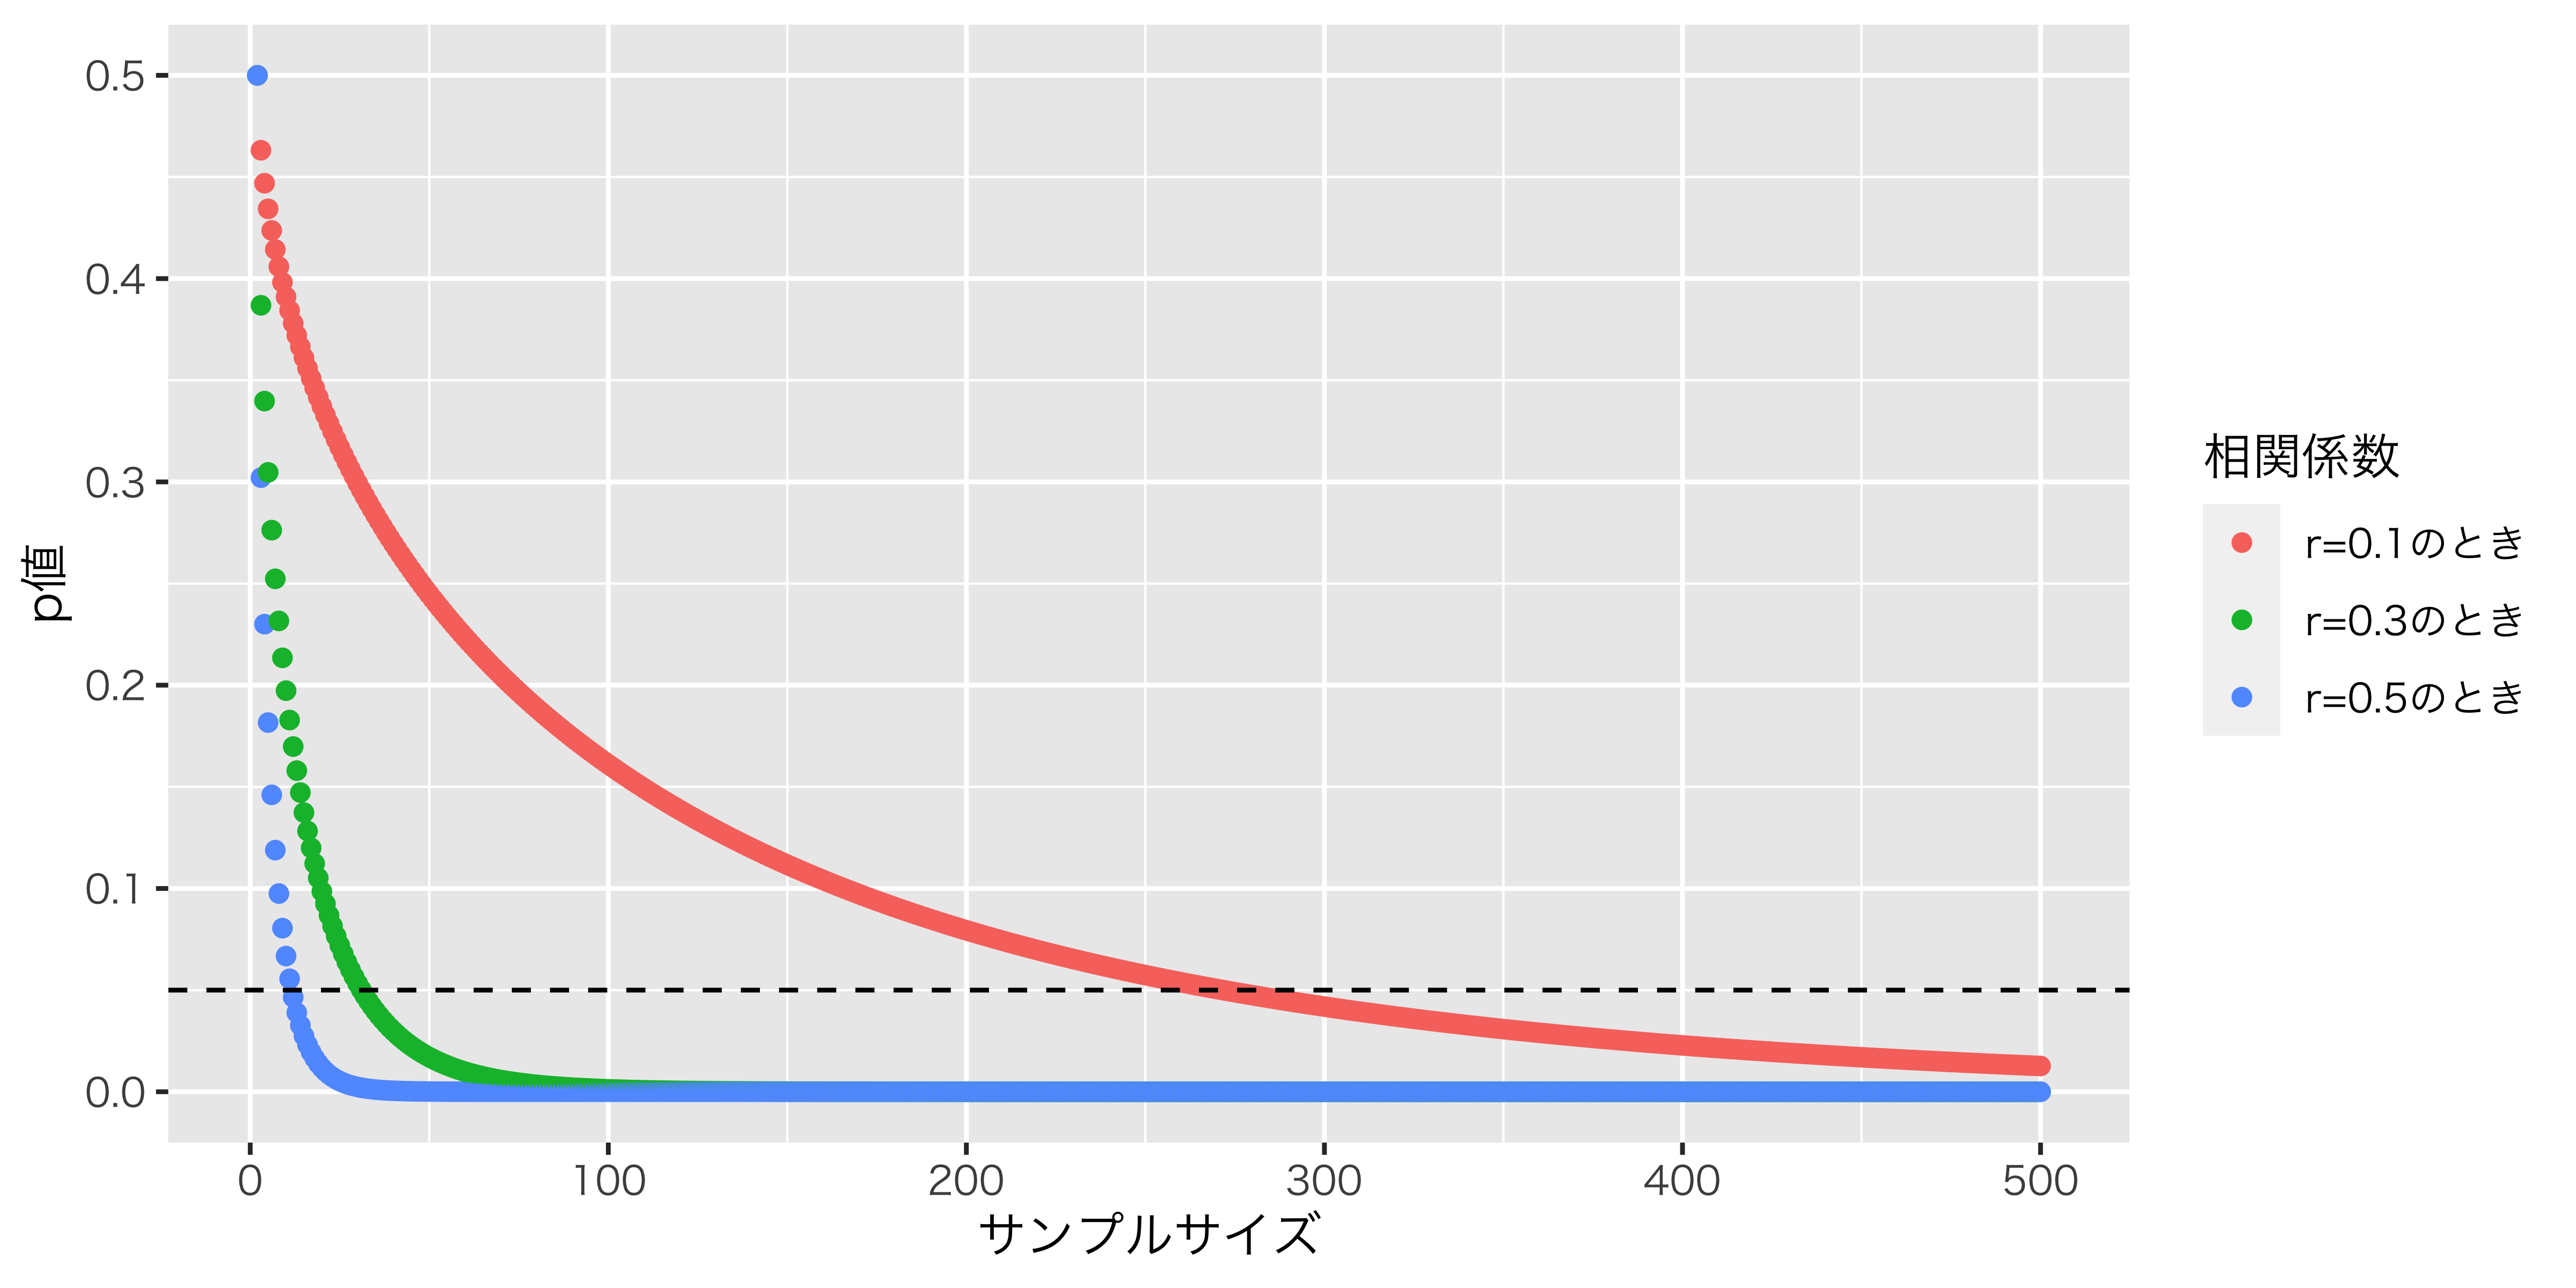
\includegraphics[keepaspectratio,width=12cm]{images/text18/Rplot18_02.png}
    \caption{サンプルサイズと$p$値の関係}
    \label{fig::18_02}
\end{figure}

この下がり方はどこからスタートするかにかかわらず同じ形ですから，判定はサンプルサイズが増えさえすればいずれ有意になるのです。これがまた，研究の実践ではおかしな風潮を読んでしまいます。つまり，\underline{有意にしたければ}サンプルサイズをたくさん取る＝頑張れば良いのです。

科学的に正しいかどうかを考えるべきシーンで，「頑張れば有意になる」といった``努力''に依存するのはおかしいことだと思いませんか。頑張った$to$有意になった$to$著者の主張が正しい，というのは，論理的ではありません。結果を自分の都合の良いように変えることは，正しい努力ではないはずです。

帰無仮説検定は，標本から母集団のことを「判定」できる優れた技術ですが，表現とその解釈に気をつけないと，科学を間違った方向に導きかねないことに注意が必要です\footnote{残念ながら，これまでの心理学の歴史の中でもこのような間違った努力がなされてきた事実があります。これらはQRPs(Questionable Research Practices：QRPs＝問題のある研究実践)と言われています。}。

\section{検定における2種類の間違い}
\label{sec::18_05}
最後に，確率を伴った判定の仕方について考えておきましょう。
先ほどから，確率を$p$値と呼んで説明してきましたが，さて，この$p$値は何を表している数字でしょうか？

\begin{itemize}
    \item 帰無仮説の生じる確率
    \item 帰無仮説の正しさを表している数字
    \item 有意差の大きさを表している数字
    \item 検定の強さを表している数字
\end{itemize}

正解は，上のどれでもない，です。意地の悪い選択肢でごめん。
上の二つの選択肢，「帰無仮説の生じる確率」「帰無仮説のただしさを表している数字」はよくある引っ掛けなのですが，仮説検定は「帰無仮説の下で・・・」という前庭から始まります。無相関検定のときに，母相関が0の世界から標本をピックアップする例をお話ししましたね。母相関の世界を前提として・・・という話なので，帰無仮説の生じる確率は100\%，帰無仮説の正しさも100\%です(だって仮定したんだから！)。

有意の程度の大きさを表す数字でもありません。確かに差が大きいとか，帰無仮説の世界から大きく離れているというようなことがあれば，検定統計量の実現値は大きくなり，$p$値は小さくなります。が，$p$値が示しているのは(帰無仮説の下での)検定統計量の出現確率であり，いわば帰無仮説という仮想空間の中での数字であって，現実の統計量について何か示す数字ではないのです。

検定の強さを表す数字，でもありません。$p$値が小さくなればなるほど，確かにレア度は増しているのですが，それは帰無仮説という仮想空間の中でのレア度であって，帰無仮説が対立仮説をどれほど打ち負かしたか，という情報を持っているわけではありません。ですから，$p$値が小さければ小さいほどすごい，などと思ってしまうと本質を見誤ります。

では検定の正しさや間違いについて，どのように考えれば良いのでしょうか。実はこれも，確率的表現の難しさがあるのです。
帰無仮説検定最後のステップでは「最初に定めた仮説が間違っているか正しいかを判断する」というのがありました。この判断の間違い方にも，2種類あるのです。つまり，「帰無仮説が正しいのに棄却してしまう」という間違い方と，「帰無仮説が正しくないのに採択してしまう」という間違い方です。

\begin{figure}[ht]
    \centering
    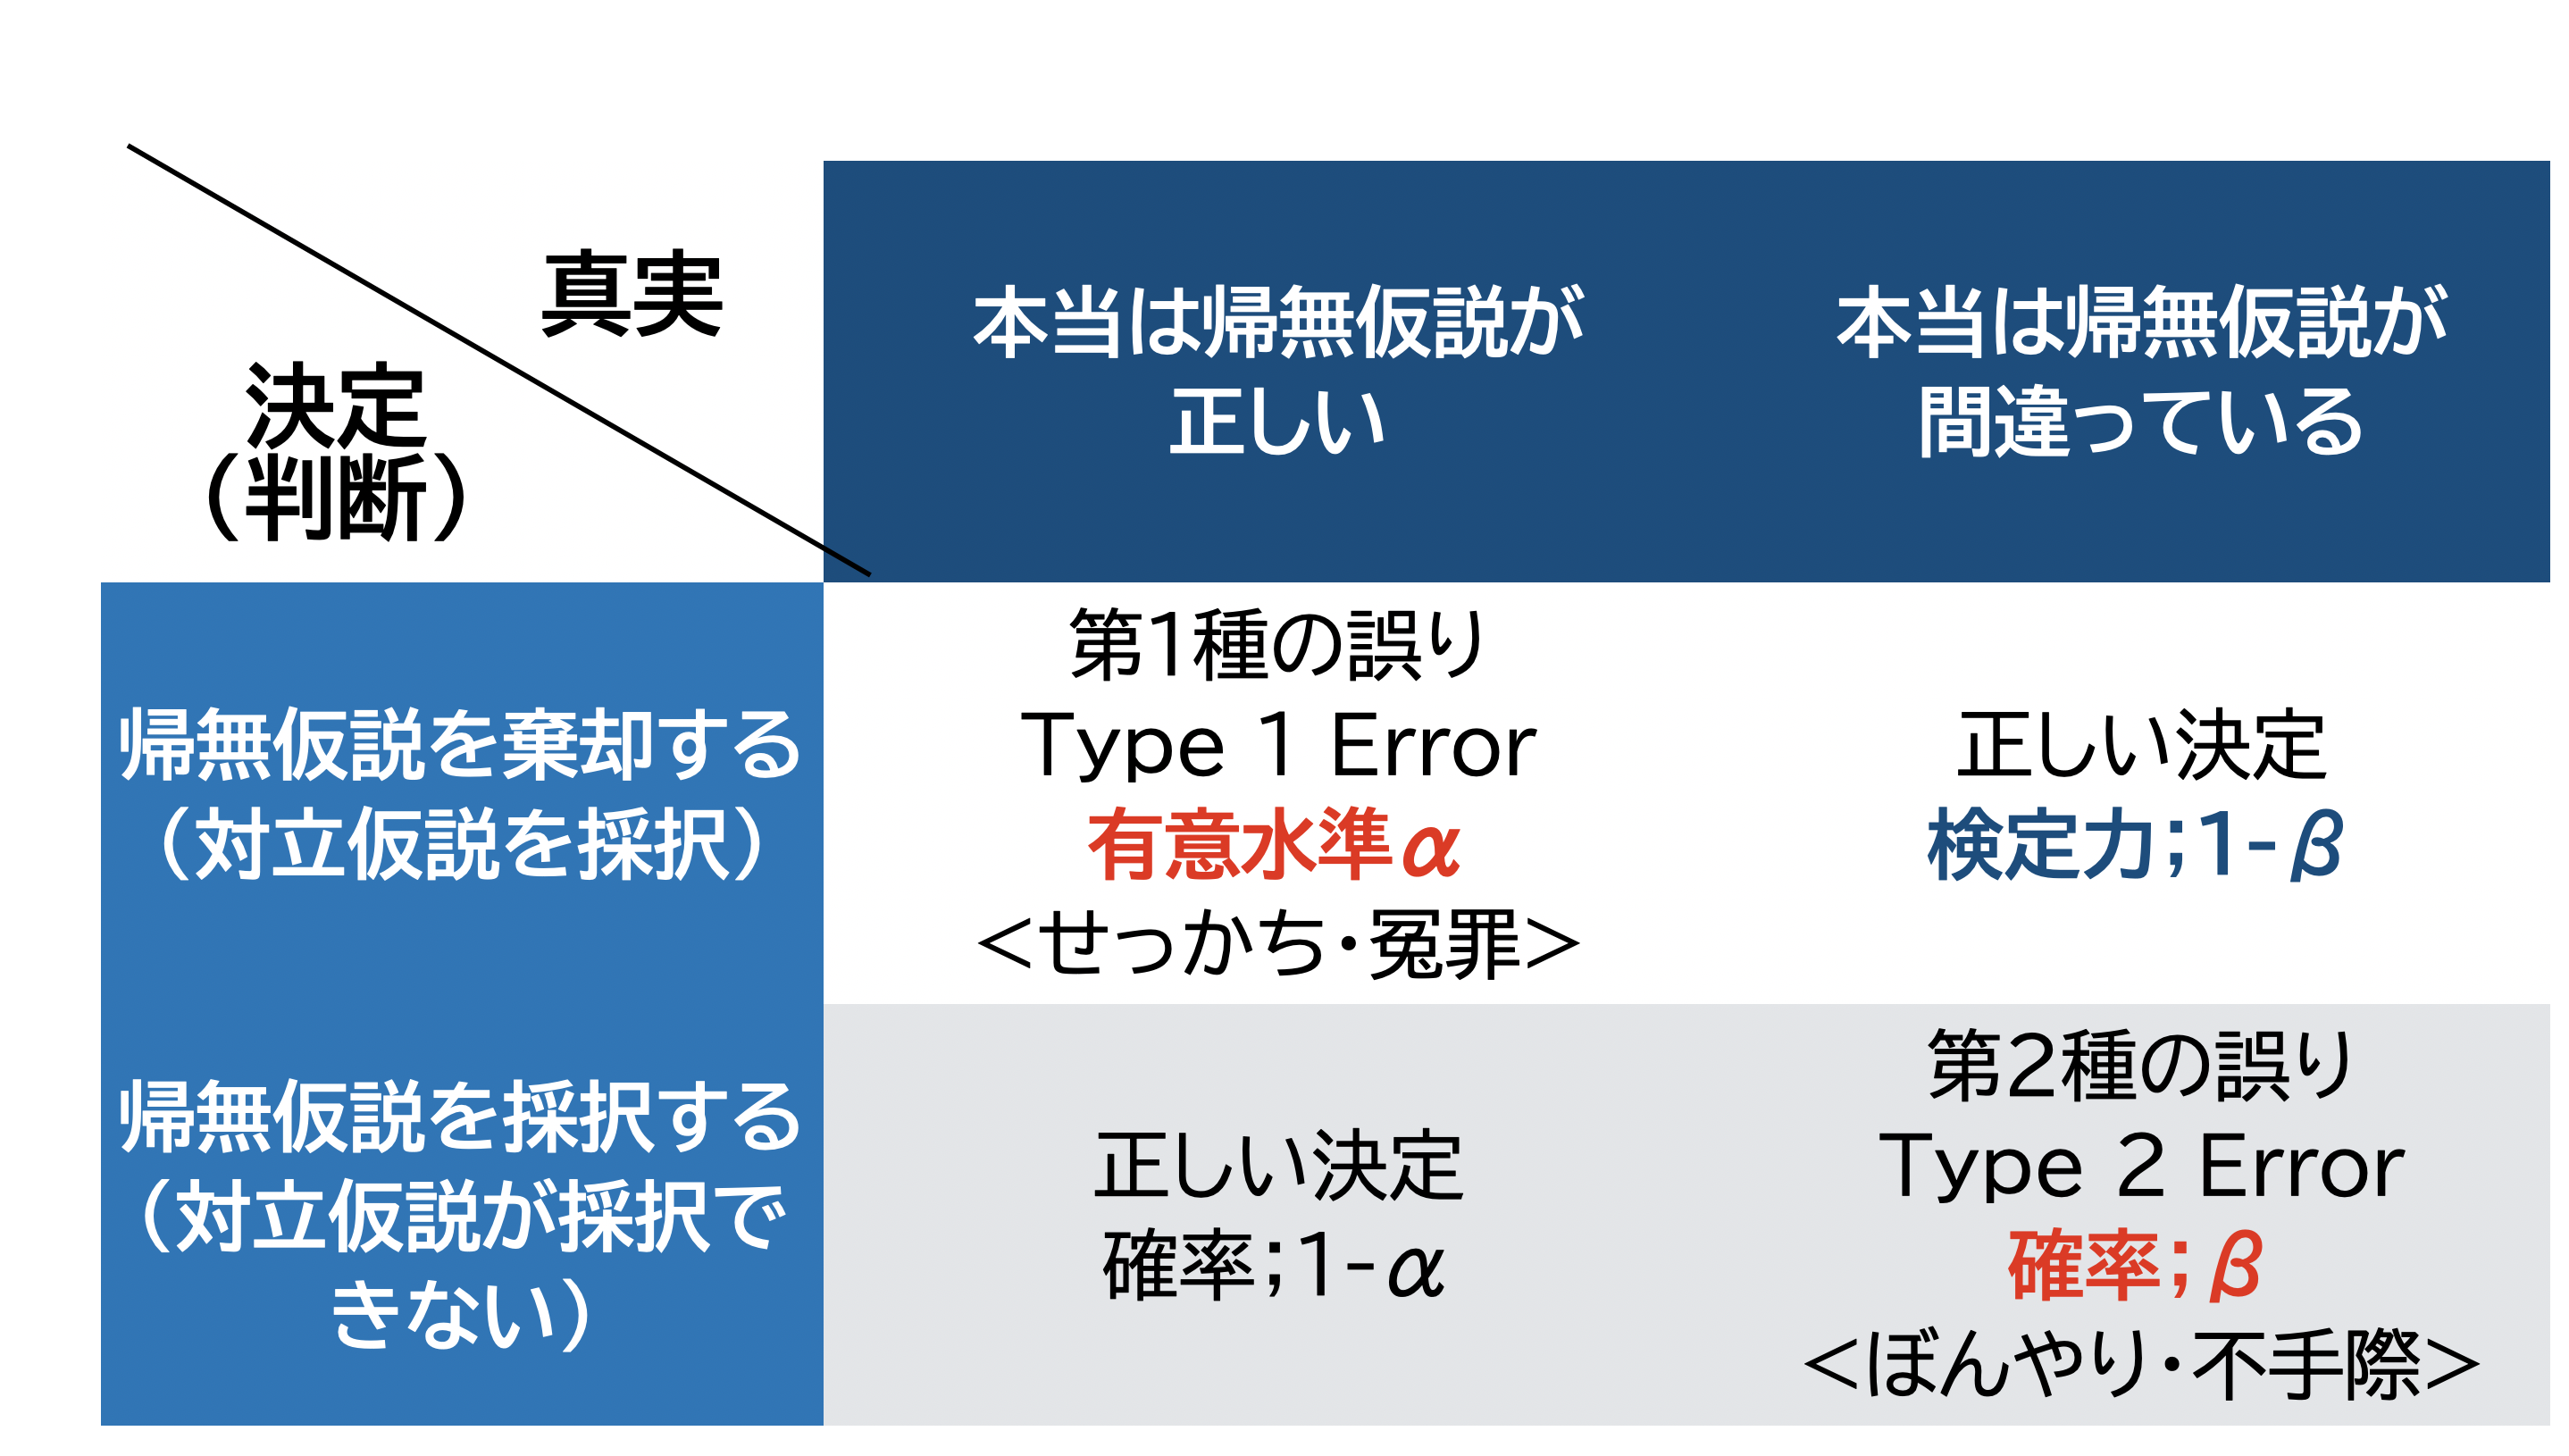
\includegraphics[keepaspectratio,width=12cm]{images/text18/slide18_01.png}
    \caption{二種類の間違い方}
    \label{fig::18_03}
\end{figure}
図\ref{fig18::13}に，間違い方の組み合わせを書いてみました。帰無仮説が正しいときに帰無仮説を採択する，帰無仮説が正しくないので帰無仮説を棄却する。これができれば正しい決定ですが，「帰無仮説が正しいのに帰無仮説を棄却する」のも「帰無仮説が正しくないのに帰無仮説を採択する」のも間違いです。
帰無仮説は差がないとか効果がない，といったNullな結論です。ここでは仮に，開発された新薬に治療効果があるかどうかを考えている，というシーンを想像してみてください。帰無仮説はこの新薬に効果がないときです。ロクな効果がないときに，帰無仮説を棄却する＝対立仮説を採択する＝効果があると言ってしまうのは，怖いことですね(患者さんに副作用など悪影響があるかも！)。このような功を焦って誤った判断をしてしまう危険な間違いを，\keyterm{第一種の誤り}Type I Errorとよび，その確率を$\alpha$で表します。実は，5\%水準で判断するというのは，この$\alpha$の確率を0.05にしたことになります。慣例では$\alpha=0.05$となっていますが，別に1\%でも10\%でも，自由に決定して構いません。どの程度の水準にするかは，この間違いを犯した時の重要さを参照しながら決めるべきことです。

一方，効果があるのに（帰無仮説が間違ってるのに)，帰無仮説を採択するのは，せっかくの効果を見抜けなかった残念なケースです。これも困った結果ではありますが，少なくとも患者に迷惑がかかるようなことはありませんよね。なので，こちらについてはひとまず間違っても実際的な問題は生じないでしょう。こちらのケースは\keyterm{第二種の誤り}Type II Errorと呼び，確率は$\beta$で表すのが一般的です。ただ，この$\beta$は帰無仮説が間違っている，つまりNull「でない」状態が，どう「である」のかわからないので，大きさを見積もることはできません。せめて，効果があるときはちゃんとあるって知りたいよね，と思いを馳せるだけです。この図\ref{fig::18_03}にある表は，列ごとに世界線が分かれていますから，右列の「帰無仮説が間違っている世界」で「帰無仮説を棄却してしまう確率」が$\beta$であれば，ちゃんと効果を見つけ出せる確率は$1-\beta$です。この$1-\beta$を\keyterm{検定力}powerといい，検定力のある分析ができているかどうかをちゃんとチェックしておくのは，研究の手続き上重要なことです。

検定力のチェックは，分析が終わった後に事後的にすることもできますし，事前にすることもできます。事前に，というのは，みたい効果がどの程度あるのかを考え，その効果をきちんと検出するにはサンプルサイズをどれぐらいにすれば良いのかを考えること，でもあります。このサンプルサイズを考えることを，\keyterm{例数設計}といいます。

帰無仮説検定において，例数設計はとても大事なことです。既に述べたように，サンプルサイズが大きくなると有意だという判断はしやすくなります。これは$p$値で判断する以上仕方のないことですが，だからと言ってそれを逆手にとって，事実よりも主張をするためにサンプルをたくさんとるのは，帰無仮説検定のハッキングのようなものです。ですので，検定をするときはまず「どの程度の効果が見込まれ，これを検証するためには何人ぐらいのサンプルをとらなければならない」と宣言してから，検定して判断するという手続きが必要です。この宣言をせずに検定をすると，「有意にするためにサンプルサイズを変えたのではないか」と批判されてしまうかもしれません。

学部の授業や卒論で行う実験で，例数設計をしたりサンプルサイズの宣言をするようなことはないかもしれませんが，学術業界では事前に学会にこの宣言を伝えてから研究に取り掛かる，事前登録制pre-registrationが導入されはじめています。


\end{document}
